
\subsubsection{模型建立}

针对问题二，本节将从颗粒间距离计算、连通性判定和蒙特卡洛模拟三个层面建立多颗粒导通概率计算模型。具体过程如下。

\textbf{步骤1：颗粒间表面距离计算}

两圆柱体A和B的轴线分别为线段$\mathbf{a}_1\mathbf{a}_2$和$\mathbf{b}_1\mathbf{b}_2$，轴线间最短距离通过三维线段距离算法计算。设参数$s, t \in [0,1]$分别表示两线段上的点：
\begin{equation}
\mathbf{p}(s) = \mathbf{a}_1 + s(\mathbf{a}_2 - \mathbf{a}_1), \quad \mathbf{q}(t) = \mathbf{b}_1 + t(\mathbf{b}_2 - \mathbf{b}_1)
\end{equation}
需求解$\min_{s,t} \|\mathbf{p}(s) - \mathbf{q}(t)\|^2$。令导数等于零，得到关于$s$和$t$的二元一次方程组，解得$s^*$和$t^*$，经裁剪至$[0,1]$后代入得轴线最短距离：
\begin{equation}
d_{\text{axis}} = \|\mathbf{p}(s^*) - \mathbf{q}(t^*)\|
\end{equation}

考虑到周期性边界条件，还需计算其中一个线段的所有27个周期镜像（在$\{-10000, 0, 10000\}^3$平移）与另一线段的距离，取最小值：
\begin{equation}
d_{\text{axis}}^{\text{per}} = \min_{\mathbf{o} \in \{-L,0,L\}^3} \|\mathbf{p}(s^*) - (\mathbf{q}(t^*) + \mathbf{o})\|
\end{equation}

两圆柱体表面之间的最短距离为轴线距离减去两个半径：
\begin{equation}
d_{\text{surf}}^{AA} = d_{\text{axis}}^{\text{per}} - 2R_A
\end{equation}
若$d_{\text{surf}}^{AA} \leq d_t = 1.8$ nm，则两颗粒之间形成导电连接。

\textbf{步骤2：基于并查集的连通性判定}

将所有$N$个颗粒视为图的节点，构建虚拟节点$N$（左电极）和$N+1$（右电极）。采用并查集数据结构维护连通关系。

颗粒$i$与左电极的连接条件为：
\begin{equation}
\min_{\mathbf{q} \in \text{seg}_i} |q_x - (-5000)| - R_A \leq d_t
\end{equation}
类似地判断与右电极的连接。若颗粒与电极连通，将对应节点与虚拟电极节点合并。

对所有$i<j$的颗粒对，计算$d_{\text{surf}}^{AA}$，若不超过$d_t$则将两节点合并。若任意时刻左电极节点与右电极节点处于同一集合（通过路径压缩的Find操作判断），则该微构体导通，可提前终止。

\textbf{步骤3：蒙特卡洛模拟}

对每种填充率独立运行$M=200$次蒙特卡洛试验。第$m$次试验中，随机生成$N$个金属A颗粒，执行连通性判定，记录导通状态$X_m \in \{0, 1\}$。导通概率的蒙特卡洛估计为：
\begin{equation}
\hat{P}_c = \frac{1}{M} \sum_{m=1}^{M} X_m
\end{equation}
估计量的标准误差为：
\begin{equation}
\text{SE}(\hat{P}_c) = \sqrt{\frac{\hat{P}_c (1 - \hat{P}_c)}{M}}
\end{equation}

综上所述，本节完成了多颗粒导通概率计算的完整模型建立，接下来将基于此进行求解。

\subsubsection{模型求解}

基于上述模型，本节分别对附件2固定配置和四种填充率进行求解。

首先分析附件2中49个颗粒的固定配置。颗粒间共计算了1176对距离，其中20对满足表面距离不超过1.8nm的连通条件。连通簇数量为17个，但没有任何一个连通簇同时触及左右两侧电极，因此该配置判定为不导通。该配置的填充率仅为0.0693\%，远低于后续发现的渗透阈值。

蒙特卡洛模拟结果如表\ref{tab:问题二结果}所示。

\begin{longtable}{>{\centering\arraybackslash}p{0.12\textwidth}>{\centering\arraybackslash}p{0.12\textwidth}>{\centering\arraybackslash}p{0.12\textwidth}>{\centering\arraybackslash}p{0.16\textwidth}>{\centering\arraybackslash}p{0.16\textwidth}}
  \caption{问题二各填充率蒙特卡洛模拟结果}
  \label{tab:问题二结果} \\
  \toprule
  填充率 & 颗粒数N & 模拟次数 & 导通次数 & 导通概率 \\
  \midrule
  \endfirsthead
  \caption{问题二各填充率蒙特卡洛模拟结果（续）} \\
  \toprule
  填充率 & 颗粒数N & 模拟次数 & 导通次数 & 导通概率 \\
  \midrule
  \endhead
  \bottomrule
  \endfoot
  0.50\% & 353 & 200 & 200 & 1.0000 \\
  0.60\% & 424 & 200 & 200 & 1.0000 \\
  0.70\% & 495 & 200 & 200 & 1.0000 \\
  1.00\% & 707 & 200 & 200 & 1.0000 \\
\end{longtable}

由表\ref{tab:问题二结果}可知，四种填充率下的导通概率均为100\%。这一结果与金属A圆柱体极高的长径比（$L_A/(2R_A) = 5000/60 \approx 83.3$）密切相关——根据渗流理论，高长径比填料的渗透阈值$\phi_c \propto 1/\alpha$，其中$\alpha$为长径比。对于长径比83的圆柱体，渗透阈值远低于0.50\%。在N=353时所有试验均导通，说明该填充率已远超渗透阈值。

\begin{figure}[ht]
  \centering
  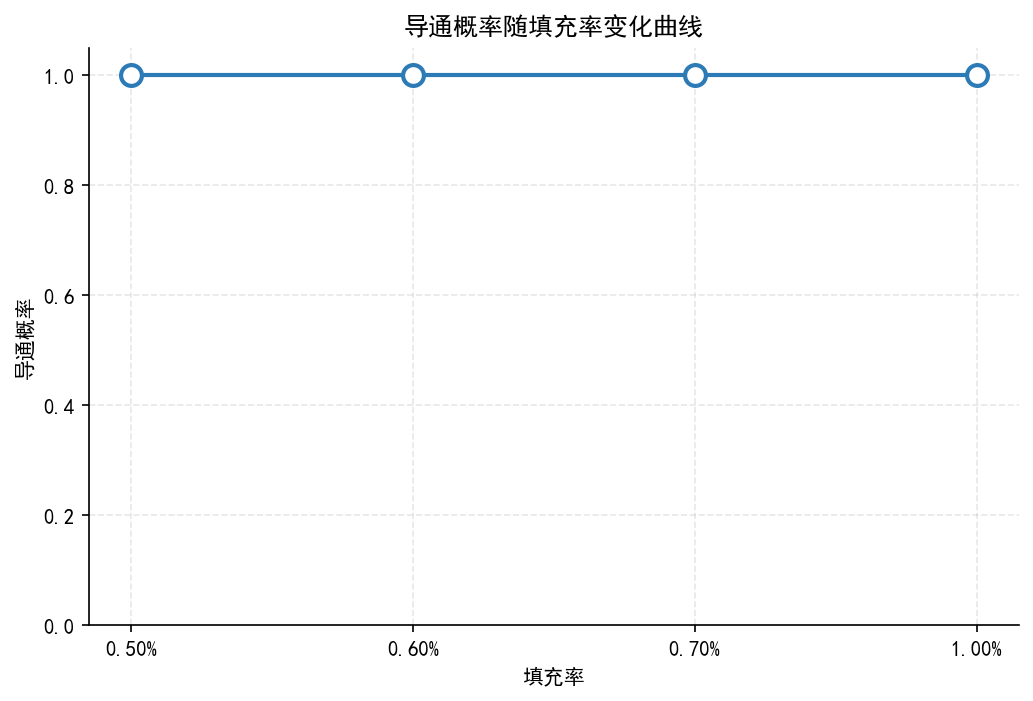
\includegraphics[width=0.8\textwidth]{../求解/问题二/图片/导通概率vs填充率曲线.png}
  \caption{导通概率随填充率变化曲线}
  \label{fig:q2_prob}
\end{figure}

\begin{figure}[ht]
  \centering
  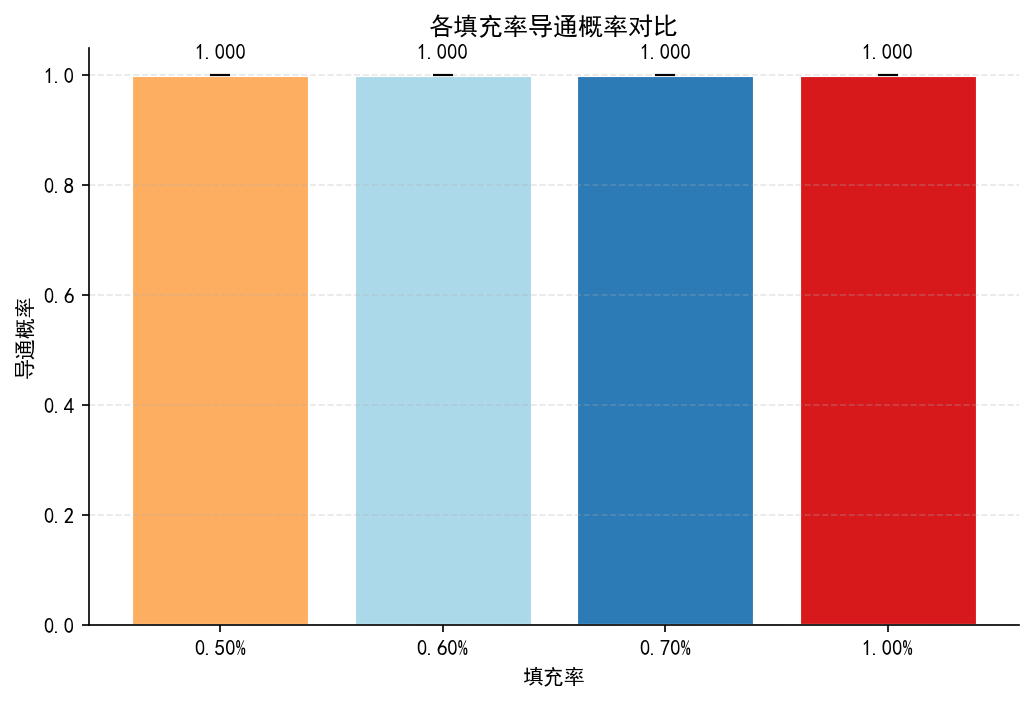
\includegraphics[width=0.8\textwidth]{../求解/问题二/图片/导通概率对比柱状图.png}
  \caption{各填充率导通概率柱状图对比}
  \label{fig:q2_bar}
\end{figure}

\begin{figure}[ht]
  \centering
  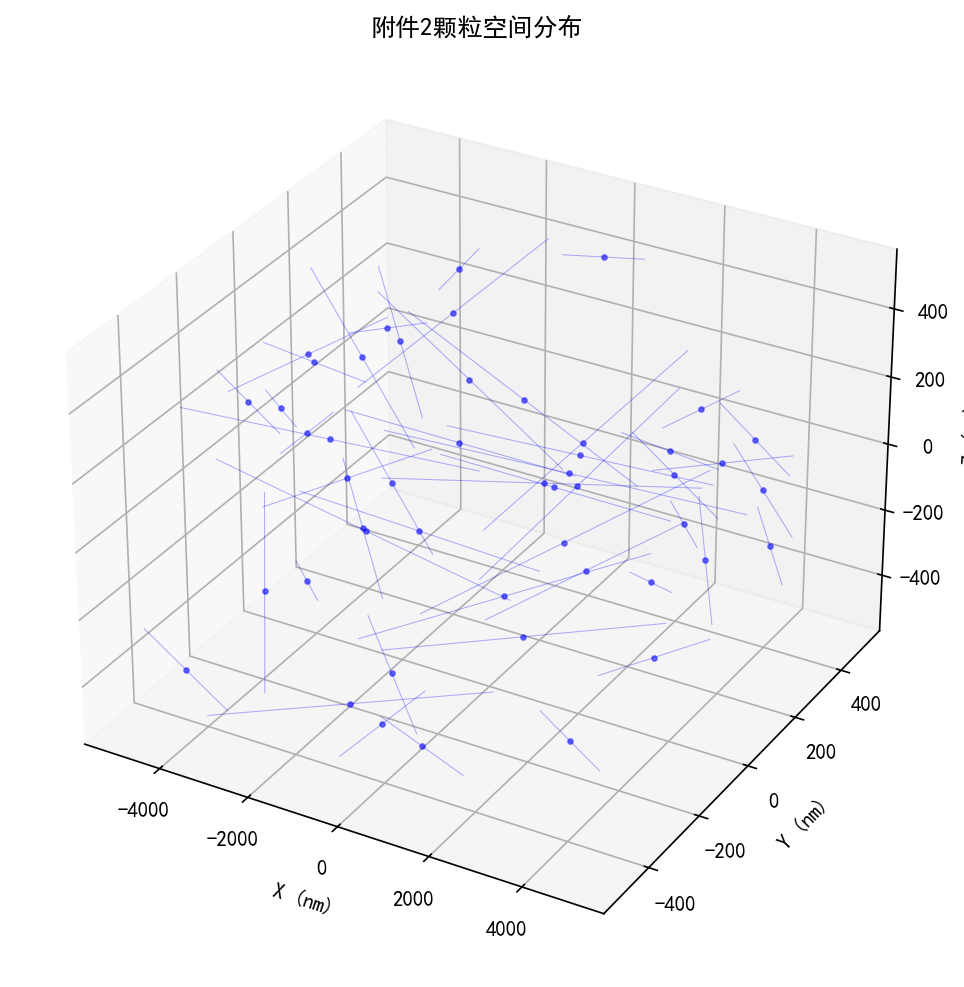
\includegraphics[width=0.8\textwidth]{../求解/问题二/图片/附件2配置连通图.png}
  \caption{附件2中49颗粒的空间分布}
  \label{fig:q2_fixed}
\end{figure}

如图\ref{fig:q2_prob}和图\ref{fig:q2_bar}所示，四种填充率下导通概率均达到1.0000，标准误差为0。附件2的49颗粒配置（如图\ref{fig:q2_fixed}）因颗粒数太少而未导通。综上所述，问题二通过蒙特卡洛模拟确定了金属A在0.50\%及以上填充率下具有100\%的导通概率。
